\documentclass{beamer}
\usepackage[utf8]{inputenc}
\usepackage[francais]{babel}
\usepackage{amsmath}
\usepackage[squaren,Gray]{SIunits}
\usepackage{numprint}
\usepackage{amsfonts}
\usepackage{amssymb}
\usepackage{graphicx}
\usepackage{mathtools}
\usepackage{mhchem}
\usepackage{hyperref}
\usepackage{varwidth}
\usetheme{Warsaw}
\title{Présentation Tâche 2:\\ création d’un flow-sheet plus détaillé et analyse paramétrique 

}
\author{Groupe 1246}
\institute{École Polytechnique de Louvain}
\date{}
\begin{document}

\begin{frame}
\titlepage
\end{frame}


\begin{frame}
\frametitle{La dernière étape du procédé}

Le procédé \textsc{Haber-Bosch}

$$\ce{N_2} + \ce{3H_2} \xrightleftharpoons \ce{2NH_3}$$

%[\mathit{endo}]{\mathit{exo}}

Supposition avec le principe de \textsc{Le Chatelier}: quand la température diminue, le rendement augmente. 

\end{frame}


\begin{frame}
\frametitle{La dernière étape du procédé}

\begin{figure}[ht!]
\centering
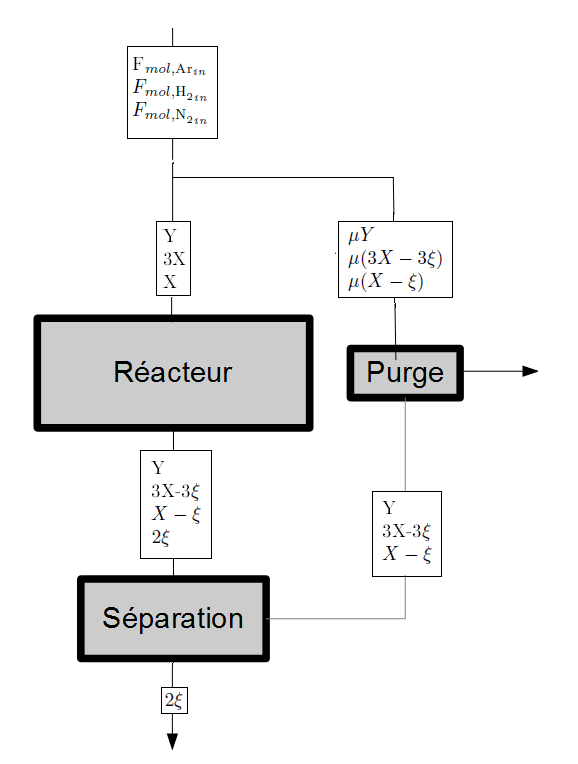
\includegraphics[scale=0.4]{Schema_synthese.png}
\caption{Aperçu des flux dans la dernière étape du procédé}
\label{Schema_synthese}
\end{figure}

\begin{table}[ht!]
\begin{center}
\begin{tabular}{|c|c|c|c|}
\hline
& \multicolumn{1}{c!{\makebox[0pt]{+}}}{\ce{N2}}
& \multicolumn{1}{c!{\makebox[0pt]{$\rightarrow$}}}{\ce{3H2}}
& \ce{2NH3} \\
\hline
$n_i$ & $X$ & $3X$ & $0$ \\
\hline
$n_f$ & $X-\xi$ & $3X - 3\xi $ & $2\xi$ \\\hline
\end{tabular}
\end{center}
\caption{Tableau d'avancement de la synthèse de l'ammoniac}
\label{Tableau}
\end{table}

\end{frame}



\begin{frame}
\frametitle{La dernière étape du procédé}

\begin{figure}[ht!]
\centering
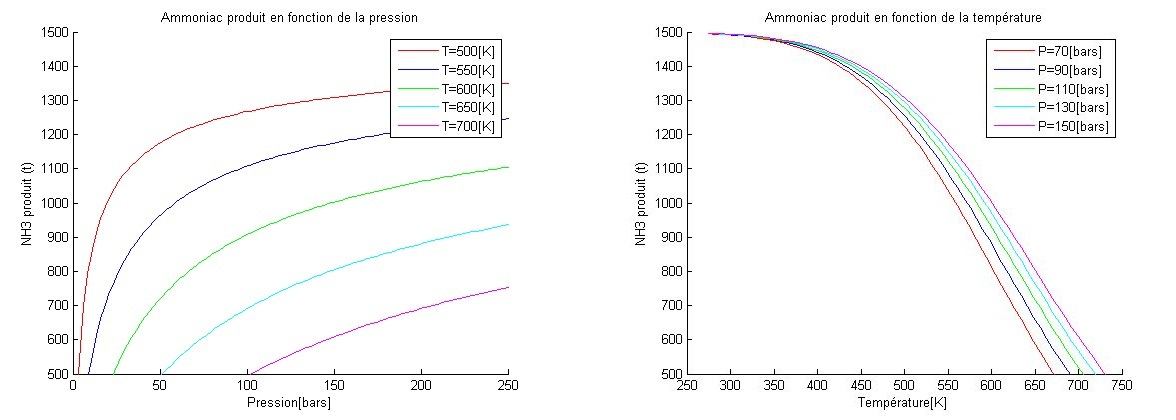
\includegraphics[scale=0.17]{fct_pression.png}
\caption{Quantité d'ammoniac produite en fonction de la température et de la pression.}
\label{fct_pression}
\end{figure}

\end{frame}




\begin{frame}
\frametitle{La dernière étape du procédé}

\begin{figure}[ht!]
\centering
\includegraphics[scale=0.5]{Aspen.jpg}
\caption{Flow-sheet réalisé avec \textsc{Apen+}}
\label{Aspen}
\end{figure}

\end{frame}



\begin{frame}
\frametitle{La dernière étape du procédé}

\begin{figure}[ht!]
\centering
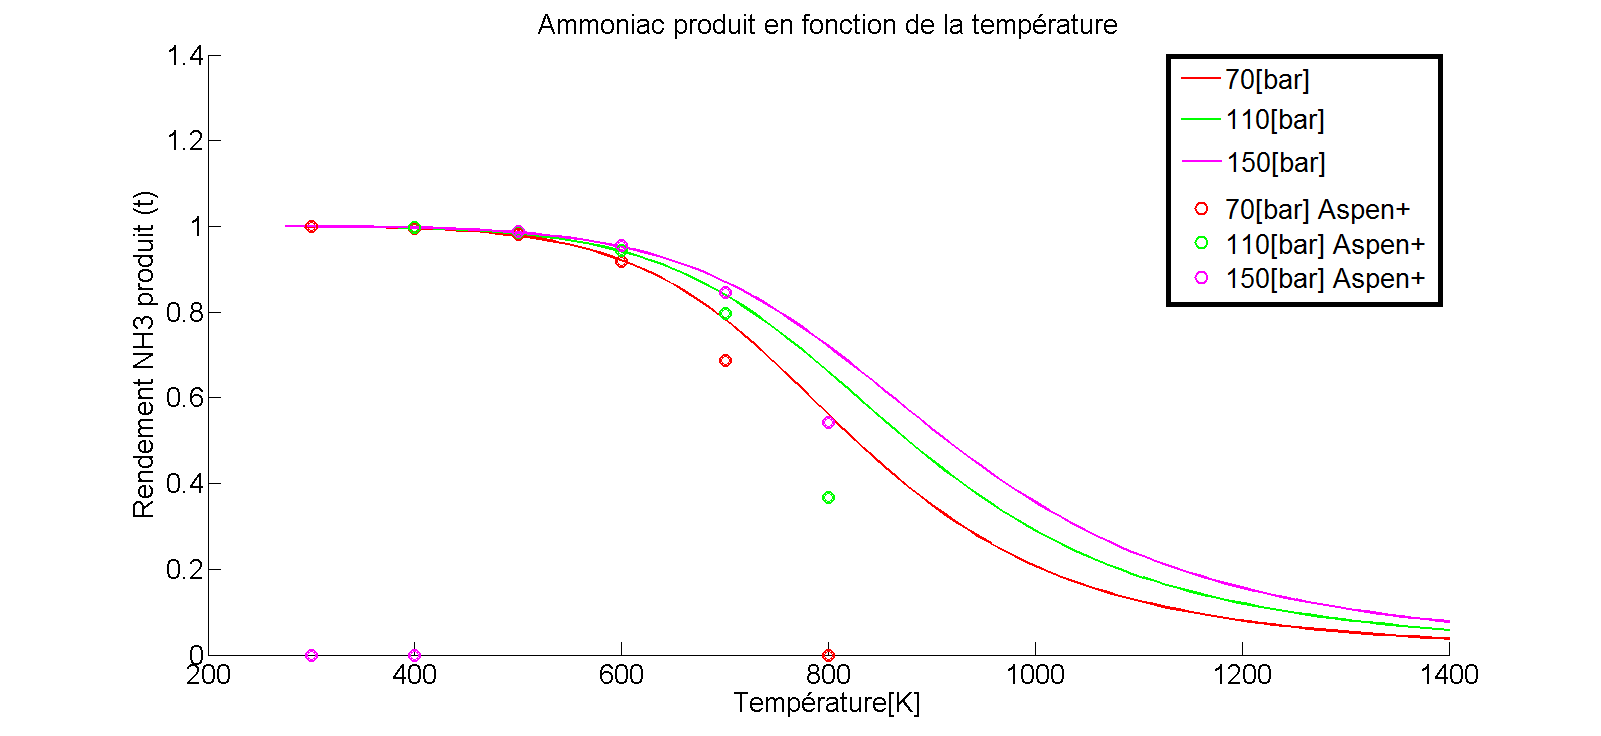
\includegraphics[scale=0.35]{GrapheCompT.png}
\caption{Rendement en fonction de la température}
\label{scheme1}
\end{figure}

\end{frame}


\begin{frame}
\frametitle{La dernière étape du procédé}

\begin{figure}[ht!]
\centering
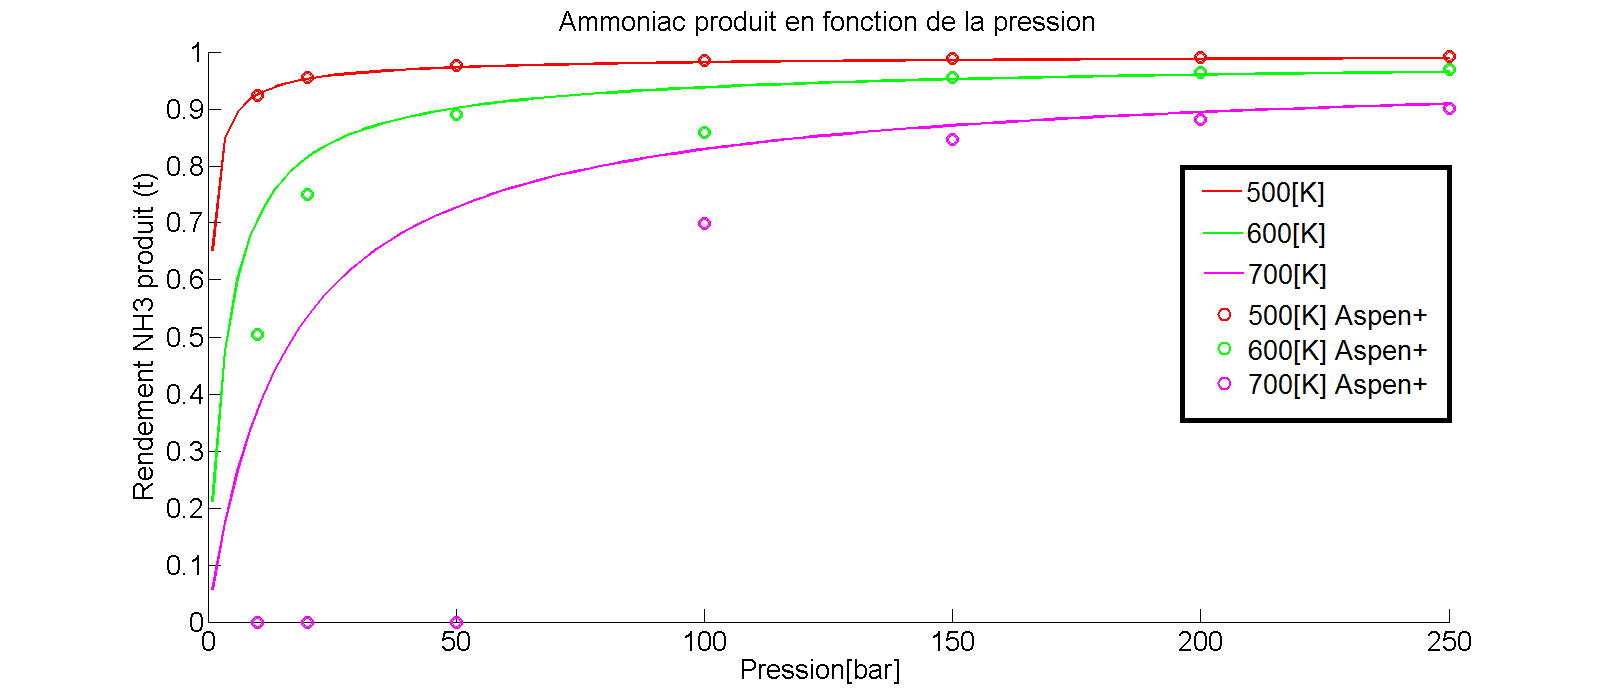
\includegraphics[scale=0.35]{GrapheCompP.png}
\caption{Rendement en fonction de la pression}
\label{scheme2}
\end{figure}

\end{frame}



\begin{frame}
\frametitle{La dernière étape du procédé}

\begin{figure}[ht!]
\centering
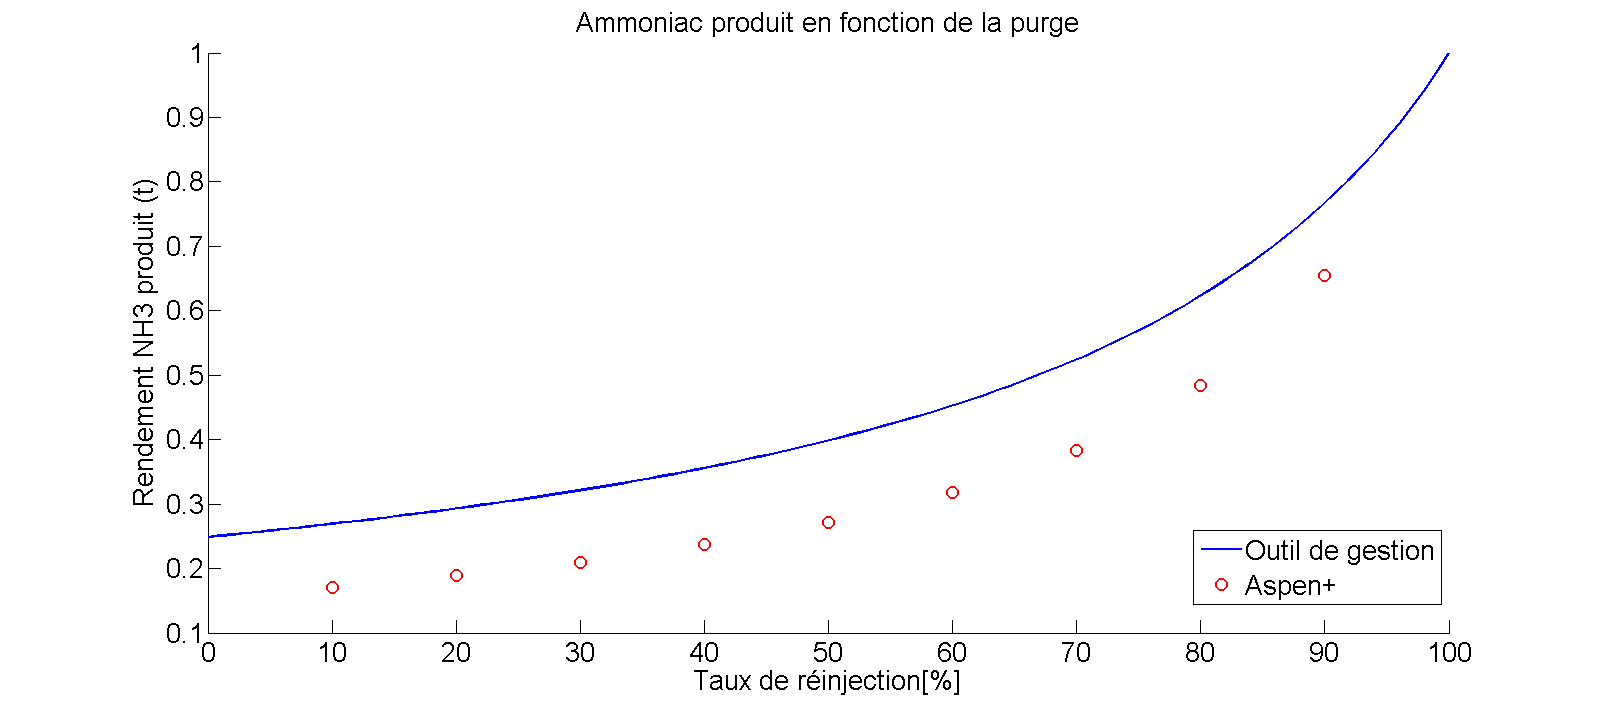
\includegraphics[scale=0.35]{GrapheCompPu.png}
\caption{Rendement en fonction du taux de purge}
\label{schemee}
\end{figure}

\end{frame}


\end{document}
